\subsection{Test boards}

% Why these board
For providing the external devices required by the testchip, and communicating with it, a master-slave architecture has been chosen.
The testchip is the slave, because it receives commands from the master for configuration and responds to reading requests.
One \gls{pcb} is designed for the master, and one for the slave.
The slave board contains the testchip and the required external devices.
The master board contains the microcontroller responsible for generating the frames for the testchip's monitoring system (section \ref{sec:comm-system-testchip}).
The master board connects to a computer for providing a user interface, reading, writing and storing the monitoring data.

% Overview of the setup
To protect the computer from \gls{esd} discharges, the two boards are isolated electrically.
Each board is powered with its own isolated battery, to avoid conducted stress propagating in the AC supply network.
The communication between the two is achieved with several optical fibers.
Optical communication is ideal because it completely isolates both boards electrically, and the fiber itself is completely immune to electrostatic discharges and more generally to electrical disturbances.
Each board packs its own set of optical to electrical converters, to make the conversion between the fiber and electrical signals.

\begin{figure}[!h]
  \centering
  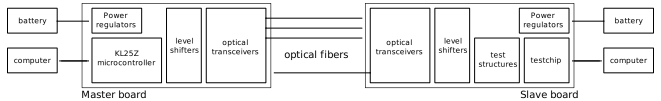
\includegraphics[width=\textwidth]{src/3/figures/boards_architecture.pdf}
  \caption{System architecture}
  \label{fig:system-board-architecture}
\end{figure}


%TODO: Picture?
